%%%%%%%%%%%%%%%%%%%%%%%%%%%%%%%%%%%%%%%%%
% Programming/Coding Assignment
% LaTeX Template
%
% This template has been downloaded from:
% http://www.latextemplates.com
%
% Original author:
% Ted Pavlic (http://www.tedpavlic.com)
%
% Note:
% The \lipsum[#] commands throughout this template generate dummy text
% to fill the template out. These commands should all be removed when 
% writing assignment content.
%
% This template uses a Perl script as an example snippet of code, most other
% languages are also usable. Configure them in the "CODE INCLUSION 
% CONFIGURATION" section.
%
%%%%%%%%%%%%%%%%%%%%%%%%%%%%%%%%%%%%%%%%%

%----------------------------------------------------------------------------------------
%	PACKAGES AND OTHER DOCUMENT CONFIGURATIONS
%----------------------------------------------------------------------------------------

\documentclass{article}

\usepackage{fancyhdr} % Required for custom headers
\usepackage{lastpage} % Required to determine the last page for the footer
\usepackage{extramarks} % Required for headers and footers
\usepackage[usenames,dvipsnames]{color} % Required for custom colors
\usepackage{graphicx} % Required to insert images
\usepackage{listings} % Required for insertion of code
\usepackage{courier} % Required for the courier font
\usepackage{lipsum} % Used for inserting dummy 'Lorem ipsum' text into the template

% Margins
\topmargin=-0.45in
\evensidemargin=0in
\oddsidemargin=0in
\textwidth=6.5in
\textheight=9.0in
\headsep=0.25in

\linespread{1.1} % Line spacing

% Set up the header and footer
\pagestyle{fancy}
\lhead{\hmwkAuthorName} % Top left header
\chead{\hmwkClass\ (\hmwkClassInstructor\ \hmwkClassTime): \hmwkTitle} % Top center head
\rhead{\firstxmark} % Top right header
\lfoot{\lastxmark} % Bottom left footer
\cfoot{} % Bottom center footer
\rfoot{Page\ \thepage\ of\ \protect\pageref{LastPage}} % Bottom right footer
\renewcommand\headrulewidth{0.4pt} % Size of the header rule
\renewcommand\footrulewidth{0.4pt} % Size of the footer rule

\setlength\parindent{0pt} % Removes all indentation from paragraphs

%----------------------------------------------------------------------------------------
%	CODE INCLUSION CONFIGURATION
%----------------------------------------------------------------------------------------

\definecolor{MyDarkGreen}{rgb}{0.0,0.4,0.0} % This is the color used for comments
\lstloadlanguages{Perl} % Load Perl syntax for listings, for a list of other languages supported see: ftp://ftp.tex.ac.uk/tex-archive/macros/latex/contrib/listings/listings.pdf
\lstset{language=Perl, % Use Perl in this example
        frame=single, % Single frame around code
        basicstyle=\small\ttfamily, % Use small true type font
        keywordstyle=[1]\color{Blue}\bf, % Perl functions bold and blue
        keywordstyle=[2]\color{Purple}, % Perl function arguments purple
        keywordstyle=[3]\color{Blue}\underbar, % Custom functions underlined and blue
        identifierstyle=, % Nothing special about identifiers                                         
        commentstyle=\usefont{T1}{pcr}{m}{sl}\color{MyDarkGreen}\small, % Comments small dark green courier font
        stringstyle=\color{Purple}, % Strings are purple
        showstringspaces=false, % Don't put marks in string spaces
        tabsize=5, % 5 spaces per tab
        %
        % Put standard Perl functions not included in the default language here
        morekeywords={rand},
        %
        % Put Perl function parameters here
        morekeywords=[2]{on, off, interp},
        %
        % Put user defined functions here
        morekeywords=[3]{test},
       	%
        morecomment=[l][\color{Blue}]{...}, % Line continuation (...) like blue comment
        numbers=left, % Line numbers on left
        firstnumber=1, % Line numbers start with line 1
        numberstyle=\tiny\color{Blue}, % Line numbers are blue and small
        stepnumber=5 % Line numbers go in steps of 5
}

% Creates a new command to include a perl script, the first parameter is the filename of the script (without .pl), the second parameter is the caption
\newcommand{\perlscript}[2]{
\begin{itemize}
\item[]\lstinputlisting[caption=#2,label=#1]{#1.pl}
\end{itemize}
}

%----------------------------------------------------------------------------------------
%	DOCUMENT STRUCTURE COMMANDS
%	Skip this unless you know what you're doing
%----------------------------------------------------------------------------------------

% Header and footer for when a page split occurs within a problem environment
\newcommand{\enterProblemHeader}[1]{
\nobreak\extramarks{#1}{#1 continued on next page\ldots}\nobreak
\nobreak\extramarks{#1 (continued)}{#1 continued on next page\ldots}\nobreak
}

% Header and footer for when a page split occurs between problem environments
\newcommand{\exitProblemHeader}[1]{
\nobreak\extramarks{#1 (continued)}{#1 continued on next page\ldots}\nobreak
\nobreak\extramarks{#1}{}\nobreak
}

\setcounter{secnumdepth}{0} % Removes default section numbers
\newcounter{homeworkProblemCounter} % Creates a counter to keep track of the number of problems

\newcommand{\homeworkProblemName}{}
\newenvironment{homeworkProblem}[1][Problem \arabic{homeworkProblemCounter}]{ % Makes a new environment called homeworkProblem which takes 1 argument (custom name) but the default is "Problem #"
\stepcounter{homeworkProblemCounter} % Increase counter for number of problems
\renewcommand{\homeworkProblemName}{#1} % Assign \homeworkProblemName the name of the problem
\section{\homeworkProblemName} % Make a section in the document with the custom problem count
\enterProblemHeader{\homeworkProblemName} % Header and footer within the environment
}{
\exitProblemHeader{\homeworkProblemName} % Header and footer after the environment
}

\newcommand{\problemAnswer}[1]{ % Defines the problem answer command with the content as the only argument
\noindent\framebox[\columnwidth][c]{\begin{minipage}{0.98\columnwidth}#1\end{minipage}} % Makes the box around the problem answer and puts the content inside
}

\newcommand{\homeworkSectionName}{}
\newenvironment{homeworkSection}[1]{ % New environment for sections within homework problems, takes 1 argument - the name of the section
\renewcommand{\homeworkSectionName}{#1} % Assign \homeworkSectionName to the name of the section from the environment argument
\subsection{\homeworkSectionName} % Make a subsection with the custom name of the subsection
\enterProblemHeader{\homeworkProblemName\ [\homeworkSectionName]} % Header and footer within the environment
}{
\enterProblemHeader{\homeworkProblemName} % Header and footer after the environment
}

%----------------------------------------------------------------------------------------
%	NAME AND CLASS SECTION
%----------------------------------------------------------------------------------------

\newcommand{\hmwkTitle}{FE - Assignment\ \#11} % Assignment title
\newcommand{\hmwkDueDate}{Monday,\ April\ 18,\ 2016} % Due date
\newcommand{\hmwkClass}{MA\ 374} % Course/class
\newcommand{\hmwkClassTime}{} % Class/lecture time
\newcommand{\hmwkClassInstructor}{} % Teacher/lecturer
\newcommand{\hmwkAuthorName}{Silvi Pandey ( 130123045 )} % Your name

%----------------------------------------------------------------------------------------
%	TITLE PAGE
%----------------------------------------------------------------------------------------

\title{
\vspace{2in}
\textmd{\textbf{\hmwkClass:\ \hmwkTitle}}\\
\normalsize\vspace{0.1in}\small{Due\ on\ \hmwkDueDate}\\
\vspace{0.1in}\large{\textit{\hmwkClassInstructor\ \hmwkClassTime}}
\vspace{3in}
}

\author{\textbf{\hmwkAuthorName}}
\date{} % Insert date here if you want it to appear below your name

%----------------------------------------------------------------------------------------

\begin{document}

\maketitle

%----------------------------------------------------------------------------------------
%	TABLE OF CONTENTS
%----------------------------------------------------------------------------------------

%\setcounter{tocdepth}{1} % Uncomment this line if you don't want subsections listed in the ToC

\newpage

\begin{center}
\textbf{PROBLEM}
\end{center}

Consider the Vasicek model :
$$dr = \beta(\mu - r)dt + \sigma dW$$
For the three parameter sets $[\beta , \mu , \sigma , r(0)]$ given by $[5.9 , 0.2 , 0.3 , 0.1]$ , $[3.9 , 0.1 , 0.3 , 0.2]$ and
$[0.1 , 0.4 , 0.11 , 0.1]$, plot the term structure up to 10 time units (i.e, plot yield versus time). Now for each of
the three parameter sets, plot yield curves versus maturity up to 500 time units for ten different values of r(0).

\begin{center}
\textbf{SOLUTION}
\end{center}
Using Monte Carlo Simulation :\\
$$\Delta r  = \beta ( \mu - r )\Delta t + \sigma \sqrt{\Delta t}Z$$
 where Z is a  normal random variate with mean 0 and variance 1.
 The paths hence were plotted using the following equation :\\
 $$r(j) = r(j-1) + \beta ( \mu - r(j-1) )\Delta t  + \sigma \sqrt{\Delta t}Z$$
 Value of $\Delta t$ taken was 0.1.\\
 
 \textbf{Part 1 (For 10 time units)}  :
 \begin{center}
 \includegraphics[width = 80mm]{Part1}
 \end{center}
 
 \textbf{Part 2 ( For 500 time units)} :\\
 \textbf{Parameter Set 1} :
 \begin{center}
 \includegraphics[width = 80mm]{Set1}
 \end{center}
 
 \textbf{Parameter Set 2} :
 \begin{center}
 \includegraphics[width = 80mm]{Set2}
 \end{center}
 
 \textbf{Parameter Set 3} :
 \begin{center}
 \includegraphics[width = 80mm]{Set3}
 \end{center}
 
 Values of r(0) taken in all the cases are :\\
 $r(0)^{new}$ = $r(0)^{old}$  + 0.01 where  $r(0)^{old}$  in the first iteration is the value of r(0) given in each set.
 
\begin{center}
\textbf{PROBLEM}
\end{center}

Consider the CIR model :
$$dr = \beta(\mu - r)dt + \sigma \sqrt{r}dW$$
For the three parameter sets $[\beta , \mu , \sigma , r(0)]$ given by $[0.02 , 0.7 , 0.02 , 0.1]$ , $[0.7 , 0.1 , 0.3 , 0.2]$ and $[0.06 , 0.09 , 0.5 , 0.02]$, plot the term structure up to 10 time units (i.e, plot yield versus time). For the parameter
set $[\beta ,\mu , \sigma]$ given by $[0.02 , 0.7 , 0.02]$ and with $r(0) = 0.1 : 0.1 : 1$, plot yield curves versus maturity for 600 time units.

\begin{center}
\textbf{SOLUTION}
\end{center}
Using Monte Carlo Simulation :\\
$$\Delta r = \beta(\mu - r)\Delta t + \sigma \sqrt{r\Delta t}Z$$
where Z is a normal random variate with mean 0 and variance 1. The paths hence were plotted using the following equation :
$$r(j) = r(j-1) + \beta (\mu -r(j-1))\Delta t +\sigma \sqrt{r(j-1)\Delta t}Z$$
Value of $\Delta t$ taken was 0.1\\

\textbf{Part 1 (For 10 time units)} :
\begin{center}
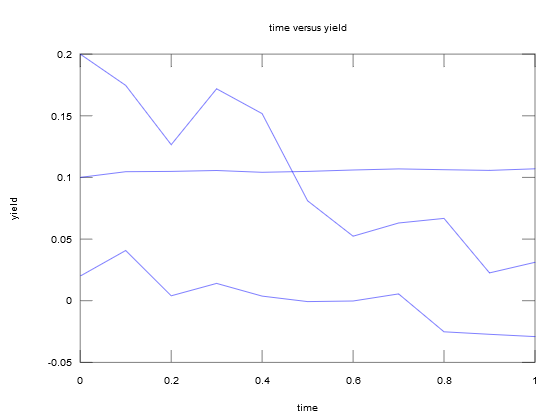
\includegraphics[width = 80mm]{Part1Q2}
\end{center}

\textbf{Part 2 (For 600 time units)} :
\begin{center}
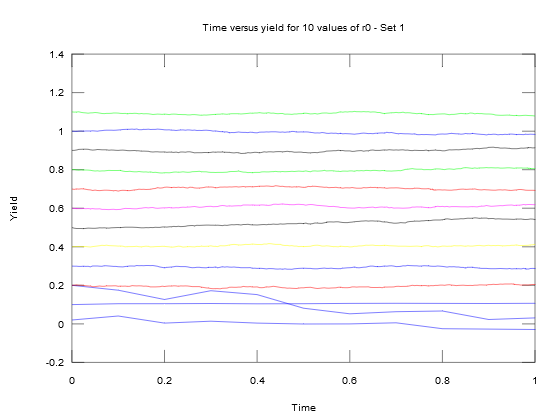
\includegraphics[width = 80mm]{Set1Q2}
\end{center}

\textbf{Observations} :\\
1. The rate of interest in the case of Vasicek's Model is more fluctuating compared to CIR model.\\
2. The rate of interest evolves almost as a constant when r(0) = 0.1\\












\end{document}